% Practice Test 11 — Florida Edition
% Questions: 30 (19 MC + 11 SA)
% Generated by scripts/generate_practice_tests.py

\begin{practiceQuestion}{1-3-q09}{mc}
\begin{questionText}
Find $k$ from the table.

\begin{center}
\begin{tabular}{|c|c|}
\hline $x$ & $y$ \\ \hline $6$ & $9$ \\ $10$ & $15$ \\ $14$ & $21$ \\ \hline
\end{tabular}
\end{center}
\end{questionText}
\choiceA{$1.5$}
\choiceB{$3$}
\choiceC{$\frac{2}{3}$}
\choiceD{$6$}
\correctAnswer{A}
\explanation{$k = \frac{9}{6} = 1.5$. Check: $\frac{15}{10} = 1.5$ and $\frac{21}{14} = 1.5$.}
\end{practiceQuestion}

\begin{practiceQuestion}{1-6-q11}{mc}
\begin{questionText}
A train travels $315$ miles in $4.5$ hours. At this rate, how far does it travel in $7$ hours?
\end{questionText}
\choiceA{$420$ miles}
\choiceB{$455$ miles}
\choiceC{$490$ miles}
\choiceD{$525$ miles}
\correctAnswer{C}
\explanation{Rate: $315 \div 4.5 = 70$ mph. In $7$ hours: $70 \times 7 = 490$ miles.}
\end{practiceQuestion}

\begin{practiceQuestion}{2-1-q13}{mc}
\begin{questionText}
Which proportion can be used to find $30\%$ of $90$?
\end{questionText}
\choiceA{$\dfrac{n}{90} = \dfrac{30}{100}$}
\choiceB{$\dfrac{30}{n} = \dfrac{90}{100}$}
\choiceC{$\dfrac{90}{n} = \dfrac{30}{100}$}
\choiceD{$\dfrac{n}{100} = \dfrac{30}{90}$}
\correctAnswer{A}
\explanation{The part $n$ is over the whole $90$, and the percent $30$ is over $100$: $\frac{n}{90} = \frac{30}{100}$.}
\end{practiceQuestion}

\begin{practiceQuestion}{2-2-q08}{mc}
\begin{questionText}
$15$ is what percent of $125$?
\end{questionText}
\choiceA{$10\%$}
\choiceB{$12\%$}
\choiceC{$15\%$}
\choiceD{$18\%$}
\correctAnswer{B}
\explanation{$\frac{15}{125} = \frac{p}{100}$. Cross-multiply: $125p = 1500$. Divide: $p = 12\%$.}
\end{practiceQuestion}

\begin{practiceQuestion}{2-6-q03}{mc}
\begin{questionText}
In the formula $I = Prt$, what does $P$ represent?
\end{questionText}
\choiceA{The percent rate}
\choiceB{The principal (starting amount)}
\choiceC{The interest earned}
\choiceD{The time in years}
\correctAnswer{B}
\explanation{$P$ stands for principal, which is the starting amount of money deposited or borrowed.}
\end{practiceQuestion}

\begin{practiceQuestion}{2-7-q09}{mc}
\begin{questionText}
If your estimate is exactly correct, what is the percent error?
\end{questionText}
\choiceA{$0\%$}
\choiceB{$1\%$}
\choiceC{$50\%$}
\choiceD{$100\%$}
\correctAnswer{A}
\explanation{If estimated $=$ actual, then $|estimated - actual| = 0$, so percent error $= 0\%$.}
\end{practiceQuestion}

\begin{practiceQuestion}{3-2-q09}{mc}
\begin{questionText}
A diver is at $-20$ feet. She rises $8$ feet. What is her new depth?
\end{questionText}
\choiceA{$-28$ feet}
\choiceB{$-12$ feet}
\choiceC{$12$ feet}
\choiceD{$28$ feet}
\correctAnswer{B}
\explanation{$(-20) + 8 = -12$. Rising from a negative position adds a positive: $20 - 8 = 12$, keep negative.}
\end{practiceQuestion}

\begin{practiceQuestion}{3-3-q08}{mc}
\begin{questionText}
What is the distance between $-9$ and $4$ on a number line?
\end{questionText}
\choiceA{$5$ units}
\choiceB{$-5$ units}
\choiceC{$13$ units}
\choiceD{$-13$ units}
\correctAnswer{C}
\explanation{Distance $= |{-9} - 4| = |{-13}| = 13$ units. Distance is always positive.}
\end{practiceQuestion}

\begin{practiceQuestion}{4-4-q27}{gmc}
\begin{questionText}
The arrays below show how $12$ tiles can be arranged. Which arrangement shows that $12 = 4 \times 3$?

\begin{center}
\begin{tikzpicture}[scale=0.5]
  % Arrangement A: 2 x 6
  \node[font=\bfseries] at (3, 3.5) {A: $2 \times 6$};
  \foreach \x in {0,...,5} {
    \foreach \y in {0,...,1} {
      \fill[funBlue!40] (\x+0.1, \y+0.1) rectangle (\x+0.9, \y+0.9);
      \draw[thick] (\x+0.1, \y+0.1) rectangle (\x+0.9, \y+0.9);
    }
  }
  % Arrangement B: 4 x 3
  \begin{scope}[xshift=8cm]
  \node[font=\bfseries] at (1.5, 5) {B: $4 \times 3$};
  \foreach \x in {0,...,2} {
    \foreach \y in {0,...,3} {
      \fill[funGreen!40] (\x+0.1, \y+0.1) rectangle (\x+0.9, \y+0.9);
      \draw[thick] (\x+0.1, \y+0.1) rectangle (\x+0.9, \y+0.9);
    }
  }
  \end{scope}
  % Arrangement C: 1 x 12
  \begin{scope}[xshift=13cm]
  \node[font=\bfseries] at (6, 1.5) {C: $1 \times 12$};
  \foreach \x in {0,...,11} {
    \fill[funOrange!40] (\x+0.1, 0.1) rectangle (\x+0.9, 0.9);
    \draw[thick] (\x+0.1, 0.1) rectangle (\x+0.9, 0.9);
  }
  \end{scope}
\end{tikzpicture}
\end{center}
\end{questionText}
\choiceA{Arrangement A}
\choiceB{Arrangement B}
\choiceC{Arrangement C}
\choiceD{All three arrangements}
\correctAnswer{B}
\explanation{Arrangement B shows $4$ rows and $3$ columns, illustrating $12 = 4 \times 3$. This connects to factoring: $12$ can be written as the product $4(3)$.}
\end{practiceQuestion}

\begin{practiceQuestion}{4-5-q30}{gsa}
\begin{questionText}
Rectangle $P$ has dimensions shown, and Rectangle $Q$ is cut out from it. Write a simplified expression for the remaining (shaded) area.

\begin{center}
\begin{tikzpicture}[scale=0.6]
  % Outer rectangle P
  \fill[funBlue!20] (0,0) rectangle (8,5);
  % Inner rectangle Q (cutout)
  \fill[white] (5,1) rectangle (7.5,4);
  \draw[thick, dashed] (5,1) rectangle (7.5,4);
  % Outer border
  \draw[thick] (0,0) rectangle (8,5);
  % Labels for P
  \node[below] at (4,0) {$5x + 2$};
  \node[left] at (0,2.5) {$3$};
  % Labels for Q
  \node at (6.25,2.5) {$Q$};
  \node[below] at (6.25,1) {$x + 1$};
  \node[right] at (7.5,2.5) {$2$};
  \node at (2.5,2.5) {\textbf{Shaded}};
\end{tikzpicture}
\end{center}
\end{questionText}
\correctAnswer{$13x + 4$}
\explanation{Area of $P$: $3(5x + 2) = 15x + 6$. Area of $Q$: $2(x + 1) = 2x + 2$. Remaining area: $(15x + 6) - (2x + 2) = 15x + 6 - 2x - 2 = 13x + 4$.}
\end{practiceQuestion}

\begin{practiceQuestion}{5-3-q22}{sa}
\begin{questionText}
Solve $2(x + 7) = -6$.
\end{questionText}
\correctAnswer{$x = -10$}
\explanation{Divide by $2$: $x + 7 = -3$. Subtract $7$: $x = -10$. Check: $2(-10 + 7) = 2(-3) = -6$ \checkmark.}
\end{practiceQuestion}

\begin{practiceQuestion}{5-4-q16}{mc}
\begin{questionText}
A student estimates that the solution to $0.48x + 3.1 = 12.7$ is about $x = 20$. Is this estimate reasonable?
\end{questionText}
\choiceA{Yes, the exact answer is $20$}
\choiceB{Yes, the exact answer is close to $20$}
\choiceC{No, the exact answer is about $10$}
\choiceD{No, the exact answer is about $33$}
\correctAnswer{A}
\explanation{Subtract $3.1$: $0.48x = 9.6$. Divide by $0.48$: $x = 20$. The estimate is exactly correct.}
\end{practiceQuestion}

\begin{practiceQuestion}{5-5-q04}{mc}
\begin{questionText}
Solve $5x - 10 \geq 25$.
\end{questionText}
\choiceA{$x \geq 3$}
\choiceB{$x \geq 7$}
\choiceC{$x \leq 7$}
\choiceD{$x \geq 35$}
\correctAnswer{B}
\explanation{Add $10$: $5x \geq 35$. Divide by $5$: $x \geq 7$.}
\end{practiceQuestion}

\begin{practiceQuestion}{5-6-q14}{mc}
\begin{questionText}
Solve $-3x + 12 \geq 0$ and describe the graph.
\end{questionText}
\choiceA{Closed circle at $4$, shade right}
\choiceB{Open circle at $4$, shade left}
\choiceC{Closed circle at $4$, shade left}
\choiceD{Closed circle at $-4$, shade right}
\correctAnswer{C}
\explanation{Subtract $12$: $-3x \geq -12$. Divide by $-3$ and flip: $x \leq 4$. Closed circle at $4$, shade left.}
\end{practiceQuestion}

\begin{practiceQuestion}{6-2-q20}{sa}
\begin{questionText}
A map uses $1$ cm $= 100$ km. You redraw at $1$ cm $= 25$ km. A distance is $3$ cm on the original. How long is it on the new map?
\end{questionText}
\correctAnswer{$12$ cm}
\explanation{Scale ratio: $\frac{100}{25} = 4$. New length: $3 \times 4 = 12$ cm.}
\end{practiceQuestion}

\begin{practiceQuestion}{6-4-q26}{gmc}
\begin{questionText}
The diagram shows a triangle with the given angle measures. Is this a valid triangle?

\begin{center}
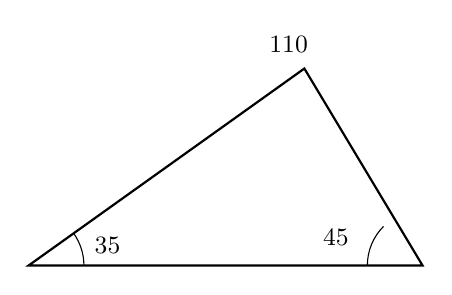
\begin{tikzpicture}[scale=1]
  \draw[thick] (0,0) -- (5,0) -- (3.5,2.5) -- cycle;
  \draw (0.7,0) arc[start angle=0,end angle=35,radius=0.7];
  \node at (1.0,0.25) {\small $35°$};
  \draw (4.3,0) arc[start angle=180,end angle=135,radius=0.7];
  \node at (3.9,0.35) {\small $45°$};
  \node at (3.3,2.8) {\small $110°$};
\end{tikzpicture}
\end{center}
\end{questionText}
\choiceA{Yes, because $35 + 45 + 110 = 190$}
\choiceB{Yes, because all angles are positive}
\choiceC{No, because the angles sum to $190°$ instead of $180°$}
\choiceD{No, because one angle is greater than $90°$}
\correctAnswer{C}
\explanation{$35 + 45 + 110 = 190 \neq 180$. Triangle angles must sum to exactly $180°$, so this triangle is not valid.}
\end{practiceQuestion}

\begin{practiceQuestion}{6-5-q29}{gsa}
\begin{questionText}
The diagram shows a cylinder with radius $4$ cm and height $9$ cm. A vertical cut is made through the center. Describe the cross-section and give its dimensions.

\begin{center}
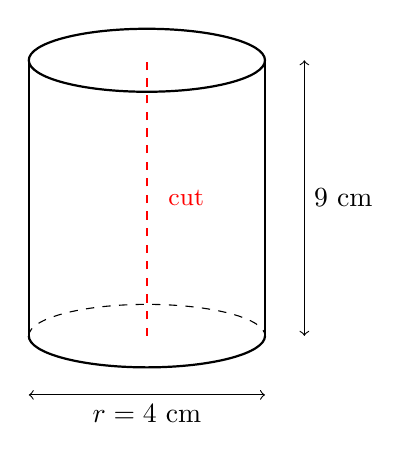
\begin{tikzpicture}[scale=0.5]
  % Cylinder
  \draw[thick] (-3,0) -- (-3,7);
  \draw[thick] (3,0) -- (3,7);
  \draw[thick] (-3,0) arc[start angle=180,end angle=360,x radius=3,y radius=0.8];
  \draw[dashed] (-3,0) arc[start angle=180,end angle=0,x radius=3,y radius=0.8];
  \draw[thick] (-3,7) arc[start angle=180,end angle=360,x radius=3,y radius=0.8];
  \draw[thick] (-3,7) arc[start angle=180,end angle=0,x radius=3,y radius=0.8];
  % Vertical cut line
  \draw[thick,red,dashed] (0,0) -- (0,7);
  \node[right,red] at (0.3,3.5) {\small cut};
  % Labels
  \draw[<->] (-3,-1.5) -- (3,-1.5);
  \node[below] at (0,-1.5) {$r = 4$ cm};
  \draw[<->] (4,0) -- (4,7);
  \node[right] at (4,3.5) {$9$ cm};
\end{tikzpicture}
\end{center}
\end{questionText}
\correctAnswer{Rectangle; $8$ cm by $9$ cm}
\explanation{A vertical cut through the center of a cylinder produces a rectangle. Width = diameter = $2 \times 4 = 8$ cm. Height = $9$ cm.}
\end{practiceQuestion}

\begin{practiceQuestion}{6-6-q30}{gsa}
\begin{questionText}
In the figure below, three angles meet on a straight line. Find the value of $x$ and the measure of each angle.

\begin{center}
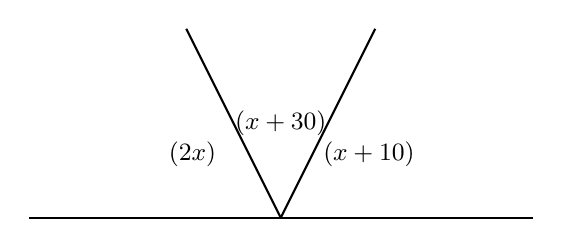
\begin{tikzpicture}[scale=0.8]
  \draw[thick] (-4,0) -- (4,0);
  \draw[thick] (0,0) -- (-1.5,3);
  \draw[thick] (0,0) -- (1.5,3);
  \node at (-1.4,1) {\small $(2x)°$};
  \node at (0,1.5) {\small $(x + 30)°$};
  \node at (1.4,1) {\small $(x + 10)°$};
\end{tikzpicture}
\end{center}
\end{questionText}
\correctAnswer{$x = 35$; angles are $70°$, $65°$, and $45°$}
\explanation{Angles on a line sum to $180°$: $2x + (x + 30) + (x + 10) = 180$. Combine: $4x + 40 = 180$. Solve: $4x = 140$, $x = 35$. Angles: $2(35) = 70°$, $35 + 30 = 65°$, $35 + 10 = 45°$. Check: $70 + 65 + 45 = 180°$ \checkmark.}
\end{practiceQuestion}

\begin{practiceQuestion}{7-1-q07}{mc}
\begin{questionText}
A circle has a radius of $3.5$ meters. What is its diameter?
\end{questionText}
\choiceA{$1.75$ m}
\choiceB{$3.5$ m}
\choiceC{$7$ m}
\choiceD{$10.5$ m}
\correctAnswer{C}
\explanation{$d = 2r = 2 \times 3.5 = 7$ m.}
\end{practiceQuestion}

\begin{practiceQuestion}{7-5-q03}{mc}
\begin{questionText}
A rectangular box is $10$ in by $6$ in by $4$ in. What is the total surface area?
\end{questionText}
\choiceA{$120$ in$^2$}
\choiceB{$240$ in$^2$}
\choiceC{$248$ in$^2$}
\choiceD{$148$ in$^2$}
\correctAnswer{C}
\explanation{$SA = 2(10 \times 6) + 2(10 \times 4) + 2(6 \times 4) = 120 + 80 + 48 = 248$ in$^2$.}
\end{practiceQuestion}

\begin{practiceQuestion}{7-6-q25}{sa}
\begin{questionText}
Two rectangular prisms have the same base of $5$ cm by $4$ cm. Prism A is $6$ cm tall and Prism B is $9$ cm tall. What is the difference in their volumes?
\end{questionText}
\correctAnswer{$60$ cm$^3$}
\explanation{$V_A = 5 \times 4 \times 6 = 120$ cm$^3$. $V_B = 5 \times 4 \times 9 = 180$ cm$^3$. Difference: $180 - 120 = 60$ cm$^3$.}
\end{practiceQuestion}

\begin{practiceQuestion}{7-7-q10}{mc}
\begin{questionText}
A cylinder has a diameter of $10$ in and a height of $6$ in. What is its volume? Use $\pi \approx 3.14$.
\end{questionText}
\choiceA{$188.4$ in$^3$}
\choiceB{$471$ in$^3$}
\choiceC{$942$ in$^3$}
\choiceD{$1{,}884$ in$^3$}
\correctAnswer{B}
\explanation{$r = 5$ in. $V = \pi r^2 h = 3.14 \times 25 \times 6 = 471$ in$^3$.}
\end{practiceQuestion}

\begin{practiceQuestion}{8-1-q25}{sa}
\begin{questionText}
A factory produces $10{,}000$ batteries per day. A sample of $200$ batteries is tested, and $8$ are defective. What percent of the sample is defective?
\end{questionText}
\correctAnswer{$4\%$}
\explanation{$\frac{8}{200} = 0.04 = 4\%$.}
\end{practiceQuestion}

\begin{practiceQuestion}{8-3-q07}{mc}
\begin{questionText}
Two box plots are drawn on the same number line. Box plot A is entirely to the right of box plot B. What does this tell you?
\end{questionText}
\choiceA{Group A has more data}
\choiceB{All values in Group A are greater than all values in Group B}
\choiceC{Group A has no overlap with Group B}
\choiceD{Both B and C}
\correctAnswer{D}
\explanation{If box plot A is entirely to the right, every value in A exceeds every value in B, so there is no overlap.}
\end{practiceQuestion}

\begin{practiceQuestion}{8-4-q23}{sa}
\begin{questionText}
Data: $100, 200, 300, 400, 500$. Find the median and the IQR.
\end{questionText}
\correctAnswer{Median $= 300$; IQR $= 200$}
\explanation{Median (3rd value) $= 300$. $Q_1 = 200$, $Q_3 = 400$. IQR $= 400 - 200 = 200$.}
\end{practiceQuestion}

\begin{practiceQuestion}{8-5-q19}{sa}
\begin{questionText}
Create a stem-and-leaf plot for: $32, 35, 41, 43, 47, 50, 52, 58$. What are the stems?
\end{questionText}
\correctAnswer{Stems: $3, 4, 5$}
\explanation{Stem $3$: leaves $2, 5$. Stem $4$: leaves $1, 3, 7$. Stem $5$: leaves $0, 2, 8$.}
\end{practiceQuestion}

\begin{practiceQuestion}{8-6-q25}{sa}
\begin{questionText}
A class of $50$ students: $20$ prefer summer, $15$ prefer winter, $10$ prefer fall, $5$ prefer spring. What percent prefer fall?
\end{questionText}
\correctAnswer{$20\%$}
\explanation{$\frac{10}{50} = 0.20 = 20\%$.}
\end{practiceQuestion}

\begin{practiceQuestion}{9-4-q28}{gmc}
\begin{questionText}
Look at the two bags below. Which bag represents a uniform probability model for drawing a marble?

\begin{center}
\begin{tikzpicture}[scale=0.65]
  % Bag 1
  \draw[thick,rounded corners=8pt] (-3,-1.5) rectangle (0,1.5);
  \node[above,font=\bfseries] at (-1.5,1.5) {Bag 1};
  \fill[funRed] (-2.3,0.5) circle (0.3);
  \fill[funRed] (-1.5,0.5) circle (0.3);
  \fill[funBlue] (-0.7,0.5) circle (0.3);
  \fill[funBlue] (-2.3,-0.5) circle (0.3);
  \fill[funGreen] (-1.5,-0.5) circle (0.3);
  \fill[funGreen] (-0.7,-0.5) circle (0.3);
  % Bag 2
  \draw[thick,rounded corners=8pt] (1,-1.5) rectangle (4,1.5);
  \node[above,font=\bfseries] at (2.5,1.5) {Bag 2};
  \fill[funRed] (1.7,0.5) circle (0.3);
  \fill[funRed] (2.5,0.5) circle (0.3);
  \fill[funRed] (3.3,0.5) circle (0.3);
  \fill[funRed] (1.7,-0.5) circle (0.3);
  \fill[funBlue] (2.5,-0.5) circle (0.3);
  \fill[funGreen] (3.3,-0.5) circle (0.3);
\end{tikzpicture}
\end{center}
\end{questionText}
\choiceA{Bag 1 only}
\choiceB{Bag 2 only}
\choiceC{Both bags}
\choiceD{Neither bag}
\correctAnswer{A}
\explanation{Bag 1 has $2$ of each color ($2$ red, $2$ blue, $2$ green), so each color is equally likely — uniform. Bag 2 has $4$ red, $1$ blue, $1$ green — non-uniform.}
\end{practiceQuestion}

\begin{practiceQuestion}{9-6-q17}{mc}
\begin{questionText}
Two spinners are spun. Spinner 1 has sections $\{1, 2, 3\}$ and Spinner 2 has sections $\{A, B\}$. What is the probability of getting $2$ and $A$?
\end{questionText}
\choiceA{$\frac{1}{3}$}
\choiceB{$\frac{1}{5}$}
\choiceC{$\frac{1}{6}$}
\choiceD{$\frac{2}{6}$}
\correctAnswer{C}
\explanation{$P(2) = \frac{1}{3}$, $P(A) = \frac{1}{2}$. $P = \frac{1}{3} \times \frac{1}{2} = \frac{1}{6}$.}
\end{practiceQuestion}

\begin{practiceQuestion}{9-7-q19}{sa}
\begin{questionText}
A simulation uses a coin flip ($50\%$ chance) to model whether it rains on a given day. In $30$ trials, rain occurs $16$ times. What is the experimental probability of rain?
\end{questionText}
\correctAnswer{$\frac{16}{30}$}
\explanation{$P = \frac{16}{30} \approx 0.533$.}
\end{practiceQuestion}
